\section*{Problem 2 - Underwater Vehicles}
\addcontentsline{toc}{section}{Problem 2 - Underwater Vehicles }
For part 2 of this assignment the focus was shifted from the satellite in space to an Underwater Vehicle. For the entirety of this part the vehicle moves at a constant depth $z=10m$ at a speed of $U=1.5m/s$ and a pitch angle of $\theta = 2.0^\circ$ and a roll angle of $\phi = 0^\circ$. While moving on a straight line the course angel was given $\chi = 30^\circ$.
\subsection*{Problem 2.1}
\addcontentsline{toc}{subsection}{Problem 2.1}
The crab angle is given by the equation:
\begin{equation}
    \beta = \chi - \psi
    \label{eq:chi}
\end{equation}

Assuming no currents and $\beta = 0$, the resulting heading is $\psi = \chi = 30^\circ$.

Another formulation for the crab angle is

\begin{equation}
    \beta = \sin^{-1}(\frac{v}{U})
    \label{eq:beta_2}
\end{equation}

Using this, the known value of U and the fact that $\beta$ is still assumed to be zero we can calculate v, resulting in $v=0$.

When it comes to the rest of the entries of the velocity vector one could choose to calculate them using basic trigonometry, using the angle between the velocity vector and the x-axis of the body frame to calculate its u and w parts. Alternatively one could choose to use the equations for rotating from flow coordinates to body coordinates from the course book \cite{Fossen2011}. 

\begin{subequations}
\label{eq:vel_vect_calc}
    \begin{align}
        u = U cos(\alpha)cos(\beta) \\
        v = U sin(\beta) \\
        w = U sin(\alpha)cos(\beta)
    \end{align}
\end{subequations}

\begin{figure}[!htb]
	\centering
	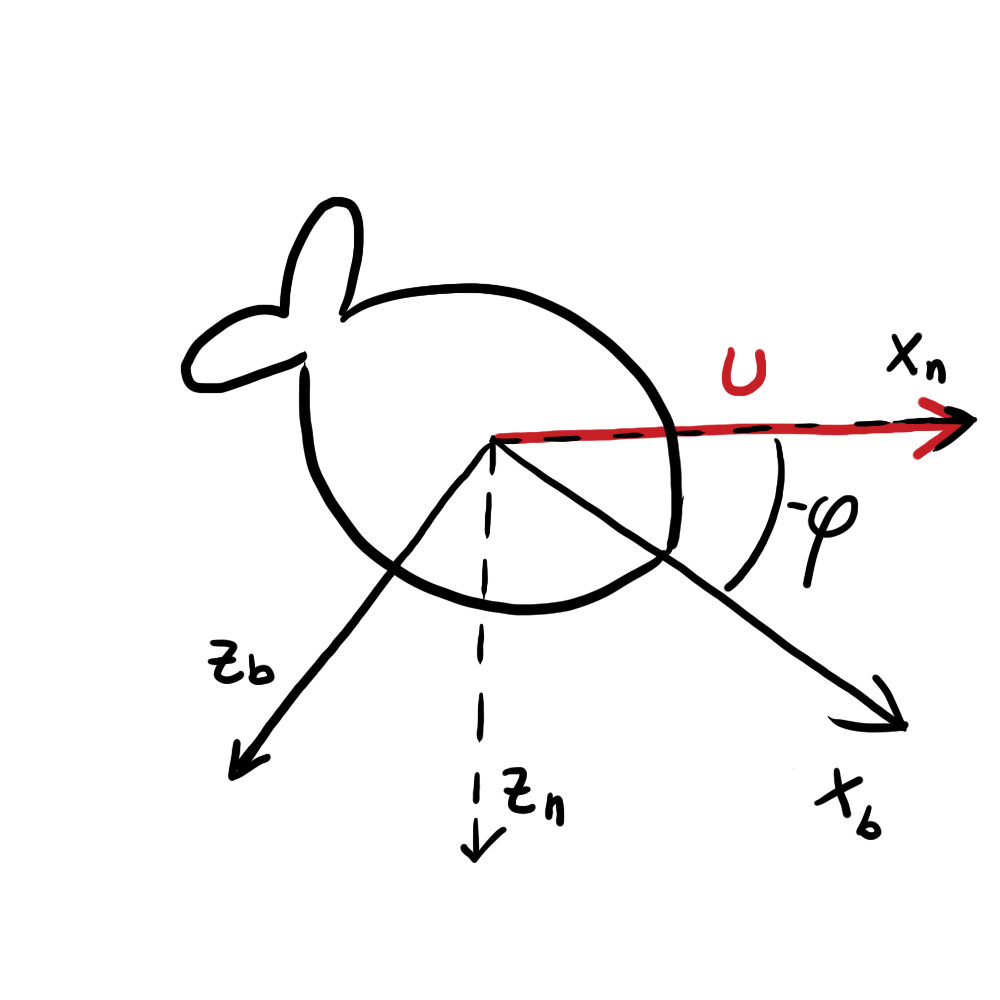
\includegraphics[width=0.70\textwidth]{figures/angleOfAttackImg.png}
	\caption{A visualization of the underwater vehicle and its velocity vector for better understanding of the calculation of the velocity.}
\label{fig:angleOfAttackImg}
\end{figure}

The equations \eqref{eq:vel_vect_calc} are equal for both methods as they represent the same transformation. For both methods, $\beta$ the crab angle, is noted to be zero.  As we know the vehicle to keep its depth unchanged the velocity vector must reside in the x-y-plane of the NED-frame, but given the tilting of the vehicle the same is not necessary true for the body frame. Both ways of calculating the body velocities means recognizing the remaining angle in question, $\alpha$ the angle of attack, as $\theta$. Equation \eqref{eq:beta_2} and \eqref{eq:vel_vect_calc} results in the same v. The calculations yielded the velocity vector

\begin{equation}
    \mathbf{v}^b_{b/n} =
    \begin{bmatrix}
		u \\
		v \\
		w
	\end{bmatrix}
	= 
	\begin{bmatrix}
		1.499 \\
		0 \\
		0.05	
	\end{bmatrix}
	\approx 
	\begin{bmatrix}
		1.5 \\
		0 \\
		0	
	\end{bmatrix}
\end{equation}

The flight path of the vehicle is given by 

\begin{equation}
    \gamma = \theta - \alpha
\end{equation}

As we already deduced $\alpha = \theta$ the result is thus $\gamma = 0^\circ$

\subsection*{Problem 2.2}
\addcontentsline{toc}{subsection}{Problem 2.2}
The vehicle was assumed to be moving on a circle with Radius $R = 100$ with the velocities assumed to be body-fixed and current-relative
\begin{equation}
\label{eq:velocity}
    \mathbf{v}^b_{b/c} = 
	\begin{bmatrix}
		u \\
		v \\
		w
	\end{bmatrix}
	= 
	\begin{bmatrix}
		U \cos( \omega t)\\
		U \sin(\omega t)\\
		0	
	\end{bmatrix}
\end{equation}

The assumption that this velocity is relative to the current is a conscious choice. We felt controlling a vehicle relative to the currents present was the most intuitive. For us it felt natural that you would maneuver a vehicle with respect to the medium that carries you and thus relative to its velocity.

Assuming no currents and knowing the speed to be constant we could calculate the turning rate for the circle by dividing one round by the time spent traveling that one round.

\begin{subequations}
    \begin{align}
        T = \frac{2\pi R}{U} \\
        r = \frac{2\pi}{T}
    \end{align}
\end{subequations}

This resulted in a turning rate $r = 0.015 rad/s$.

$\boldsymbol{\omega}$ is defined a vector, 

\begin{equation}
    \boldsymbol{\omega} =
    \begin{bmatrix}
        p \\
        q \\
        r \\
    \end{bmatrix}
\end{equation}

It is then strange that $\boldsymbol{\omega}$ is fed into trigonometric functions the way it is in \eqref{eq:velocity}. For this to hold, we need a numerical value to represent $\boldsymbol{\omega}$. Assuming our only rotation is about the z-axis, we can approximate p and q to zero, making $\omega = r = 0.015$.

With our constant velocity, we can calculate $\beta$ using \eqref{eq:beta_2}. The result is thus $\beta = \omega t$, meaning $\beta$ is changing with time. This is because, while the vehicle is moving in a circular pattern as a result of its changing velocity, the heading of the vehicle is not. How the vehicle is able to move in all directions without turning like some sort of kolibri, is unknown to us. Specifications of the vehicle on that front have not been provided. 

\begin{figure}[!htb]
	\centering
	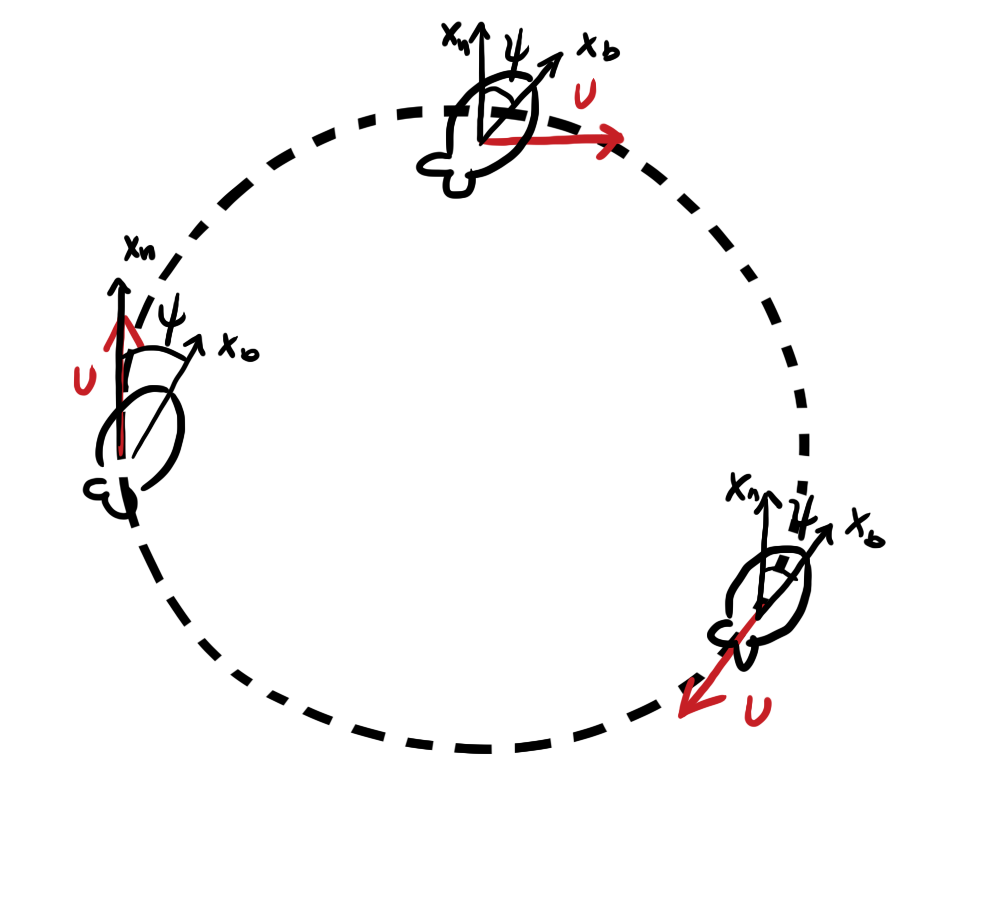
\includegraphics[width=0.70\textwidth]{figures/circleWithU.png}
	\caption{.}
\label{fig:circleWithU}
\end{figure}

\subsection*{Problem 2.3}
\addcontentsline{toc}{subsection}{Problem 2.3}

Still moving on the circle, the vehicle would now be exposed to a current with given speed $U_c = 0.6$ and directions $\alpha_c = 10^\circ$ and $\beta_c = 45^\circ$ in the vertical and horizontal plane respectively.

From the text book \cite{Fossen2011} we have the equation

\begin{equation}
    \begin{aligned}
    \mathbf{v}_{c/n}^n 
    =
    \begin{bmatrix}
    U_c \cos(\alpha_c) \cos(\beta_c) \\
    U_c \sin(\beta_c) \\
    U_c \sin(\alpha_c) \cos(\beta_c)\\
    \end{bmatrix}
    \label{eq:v_n_c}
    \end{aligned}
\end{equation}

which returns the velocity of the current, relative to NED and given in NED. $\mathbf{v^n_{c/n}} = [0.418 0.424 0.074]^\top$ with the given $\alpha_c$ and $\beta_c$. 

Relative velocities are given by

\begin{equation}
    \boldsymbol{v}_r = \boldsymbol{v}_{b/c} = \boldsymbol{v}_{b/n} + \boldsymbol{v}_{c/n}
    \label{eq:v_r}
\end{equation}

However, we already made the assumption that the velocity of the body relative to the current $\mathbf{v}_{b/c}$, was the velocity provided us in \eqref{eq:velocity}. Calculations are therefore not needed to find it. Finding the velocity vector of the body relative to NED, however, will require adding the current velocity to the given body velocity

\begin{equation}
    \mathbf{v}^n_{b/n} = \mathbf{R}_b^n(\Theta^n_b)\mathbf{v}_{b/c}^b + \mathbf{v}^n_{c/n}
\end{equation}

\todo{Er dette riktig $\Theta$??}
